%!TEX root = ../prueba.tex

\section{Arquitectura Física}
El sistema utilizará una arquitectura cliente - servidor. La parte del cliente será programada bajo el siguiente esquema(el cual puede se puede apreciar mejor en la figura \ref{fig:arqFisica}), para la parte móvil que está encargada de permitir a un usuario realizar pedidos o buscar una cafetería, entre otros requerimientos que pueden ser consultados en el siguiente capítulo, será programada utilizando el SDK para Dispositivos Móviles Android, esta aplicación se comunicará con el servidor mediante el protocolo HTTP. El servidor hará las búsquedas necesarias en la base de datos y devolverá una respuesta utilizando la especificación REST.\\

Para los usuarios que requieren subir información al sistema acerca del inventario, catálogo de productos, promociones y otros requerimientos que corresponden a un cliente web o de escritorio se utilizará el framework para front - end Angular en su versión 6 para aplicaciones web. Este cliente realizará peticiones HTTP al servidor el cual procesará los datos correspondientes y regresará una respuesta utilizando la especificación de REST.\\

\begin{figure}[hbtp!]
	\begin{center}
		\fbox{\includegraphics[width=0.5\textwidth]{img/arq_fisica}}
		\caption{Arquitectura Física del Sistema}
		\label{fig:arqFisica}
	\end{center}
\end{figure}

Para el almacenamiento de los datos del sistema se utilizará el gestor \href{https://www.postgresql.org}{Postgresql} por las siguientes ventajas:
	\begin{Citemize}
		\item Es open source.
		\item Provee de un lenguaje avanzado para la programación de store procedures, triggers y funciones.
		\item Soporta una gran cantidad de sentencias del standard SQL.
		\item Es estable y confiable.
		\item Diseñado para ambientes de alto volumen. 
	\end{Citemize}

\section{Módulos}

Con el fin de facilitar la tarea priorizar las necesidades del cliente para la creación del Prioritized Product Backlog, el sistema fue divido por módulos los cuales deberán mantener una estrecha colaboración pero ser independientes entre si. Los módulos del sistema se pueden observar en la figura \ref{fig:modulos} y a continuación se describe brevemente en qué consisten y los stakeholders para los que fue planteado. Para representar a los módulos del sistema se utilizaron paquetes siguiendo la especificación de la \href{https://www.omg.org}{OMG} para UML.


\begin{figure}[hbtp!]
	\begin{center}
		\fbox{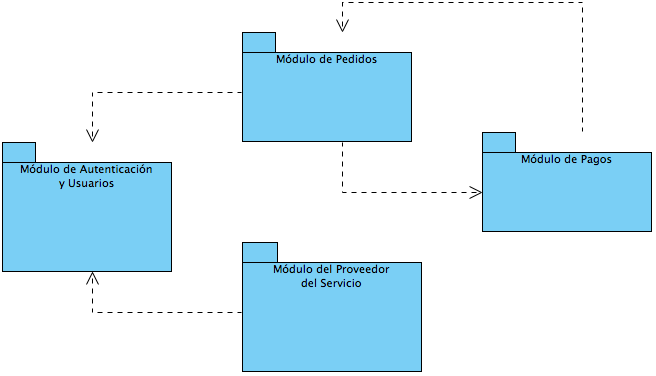
\includegraphics[width=0.5\textwidth]{img/modulos_sistema}}
		\caption{Módulos del Sistema}
		\label{fig:modulos}
	\end{center}
\end{figure}

\begin{description}
	\item[Módulo de Autenticación y Usuarios:] Este módulo tiene como principal propósito albergar la información de los usuarios que utilizan la aplicación así como de proveer de un mecanismo que permita la autenticación de usuarios y la presentación de información de acuerdo al rol o roles del usuario.
	\item[Módulo del Proveedor del Servicio:] Este módulo está pensado para ser utilizado por el personal de la cafetería y está pensado para que se administren los pedidos de los clientes. El módulo utilizará características de un dispositivo móvil o de una aplicación web según convenga la necesidad que debe cubrir.
	\item[Módulo del Cliente:] Este módulo está pensado para ser utilizado por cualquier persona que desee realizar algún pedido a una cafetería..
	\item[Módulo de Pagos:] Este módulo tiene como propósito gestionar los pagos de los clientes por el servicio utilizando transacciones en línea utilizando la API de PayPal.
\end{description}
